\documentclass{article}
\usepackage[utf8]{inputenc}
\usepackage[ukrainian]{babel}
\PassOptionsToPackage{hyphens}{url}\usepackage{hyperref}
\title{Прикладні алгоритми. Завдання 2, звіт}
\author{Михайло Голуб}
\usepackage{graphicx}
\graphicspath{ {./images/} }
\begin{document}
\maketitle
\newpage

\textbf{Реалізація класу граф:}\\\indent

Створено клас \textit{Graph} що при ініціалізації приймає на вхід матрицю суміжності ребер. Цей клас має наступні методи:
\begin{itemize}
\item[] \textbf{\textit{to\_ll}} -- повертає масив списків зв'язності;
\item[] \textbf{\textit{clear}} -- встановлює усі клітинки матриці в False;
\item[] \textbf{\textit{from\_ll}} -- створює нову матрицю зв'язності з масиву списків зв'язності;
\item[] \textbf{\textit{add\_vertice}} -- додає одну колонку та один рядок в матрицю суміжності;
\item[] \textbf{\textit{add\_edge}} -- встановлює відповідну пару клітинок в True;
\item[] \textbf{\textit{remove\_vertice}} -- видаляє колонку та рядок з вказаним індексом;
\item[] \textbf{\textit{remove\_edge}} -- встановлює відповідну пару клітинок в False.\\\\
\end{itemize}

\textbf{Реалізація інших класів:}\\\indent

Клас \textit{OrientedGraph} є нащадком (не дитиною; від англ. inherit -- наслідувати / успадковувати) \textit{Graph} з перевизначенням додання та видалення ребер: значення встановлюється не для пари клітинок, а для однієї клітинки.\\\indent
Клас \textit{WeightedGraph} є нащадком \textit{Graph} з перевизначенням методів: методи працюють не з булевими значеннями, а з числовими.\\\indent

Клас \textit{OrientedWeightedGraph} є нащадком \textit{WeightedGraph} з перевизначенням додання та видалення ребер: значення встановлюється не для пари клітинок, а для однієї клітинки.\\\\\indent

\textbf{Реалізація рандомізованих класів:}\\\indent

Класи \textit{RandomGraph, RandomOrientedGraph, RandomWeightedGraph, RandomOrienedWeightedGraph} є нащадками відповідних класів з перевизначенням \textit{\_\_init\_\_}: створюється пуста (заповнена False) матриця суміжності потрібного розміру, і через неї проходить цикл що з вказаною ймовірністю записує True або випадкове число. Для того щоб в неорієнтованих графах кожне ребро було пройдено циклом лише один раз, ітератор другої координати працює від i до n, де i -- позиція ітератора першої координати та n -- кількість вершин. В орієнтованих графах обидва ітератори працюють від 0 до n



\pagebreak
\textbf{Тестування швидкості роботи:}\\\indent

Дядько Фестер (Аддамс), представник класу \textit{SkilledTester}, проводить тестування наступним чином: генерує вказану кількість випадкових графів, виконує на ній потрібну операцію і записує час роботи. Тестуються виключно неорієнтовані незважені графи, оскільки різниця складності роботи методів знехтовно мала. На графіках вказано час роботи в мс в залежності від кількості вершин\indent
\newpage

Результати тестування \textit{add\_vertice}:\indent
\begin{center}
    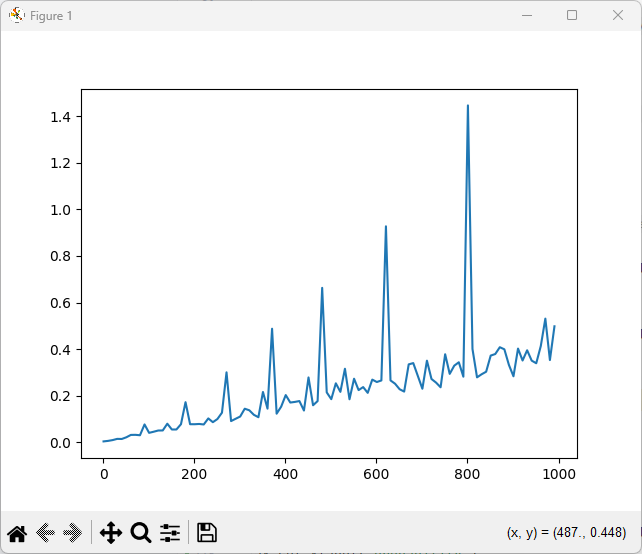
\includegraphics[width=125mm]{newvertice}
\end{center}

Явно видно, що складність методу співпадає з очікуваною складністю O(n). Проте, видно значні відхилення від прямої, скоріше за все це пов'язано з випадковою природою графів, що тестуються.\\\indent
\newpage

Результати тестування \textit{add\_edge}:
\begin{center}
    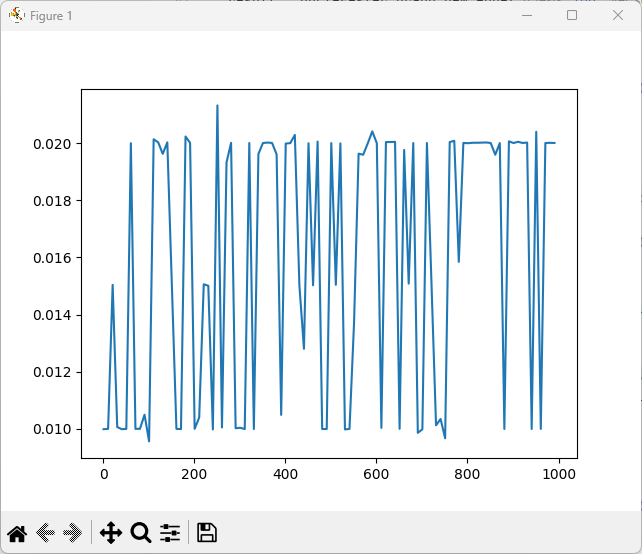
\includegraphics[width=125mm]{newedge}
\end{center}\indent

Цей метод виконується за час від 90мкс до 30мкс, що співпадає з очікуваною складністю O(1). Видалення ребер працює так само, лише записує в клітинки False замість True, тож час роботи додання та видалення ребра однаковий.
\newpage

Результати тестування \textit{rem\_vertice}:
\begin{center}
    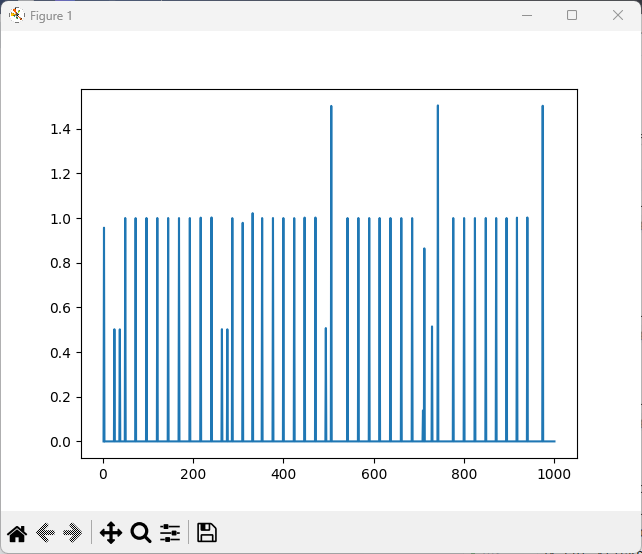
\includegraphics[width=125mm]{remvertice}
\end{center}\indent


Цей метод виконується моментально, або за час менший 2мс, отримана складність -- O(1). Очікувана складність O($n^2$) не співпадає з отриманими даними, оскільки Python може видалити рядок та стовпець матриці суміжності не перестворюючи її.
\newpage

Результати тестування \textit{to\_ll}:
\begin{center}
    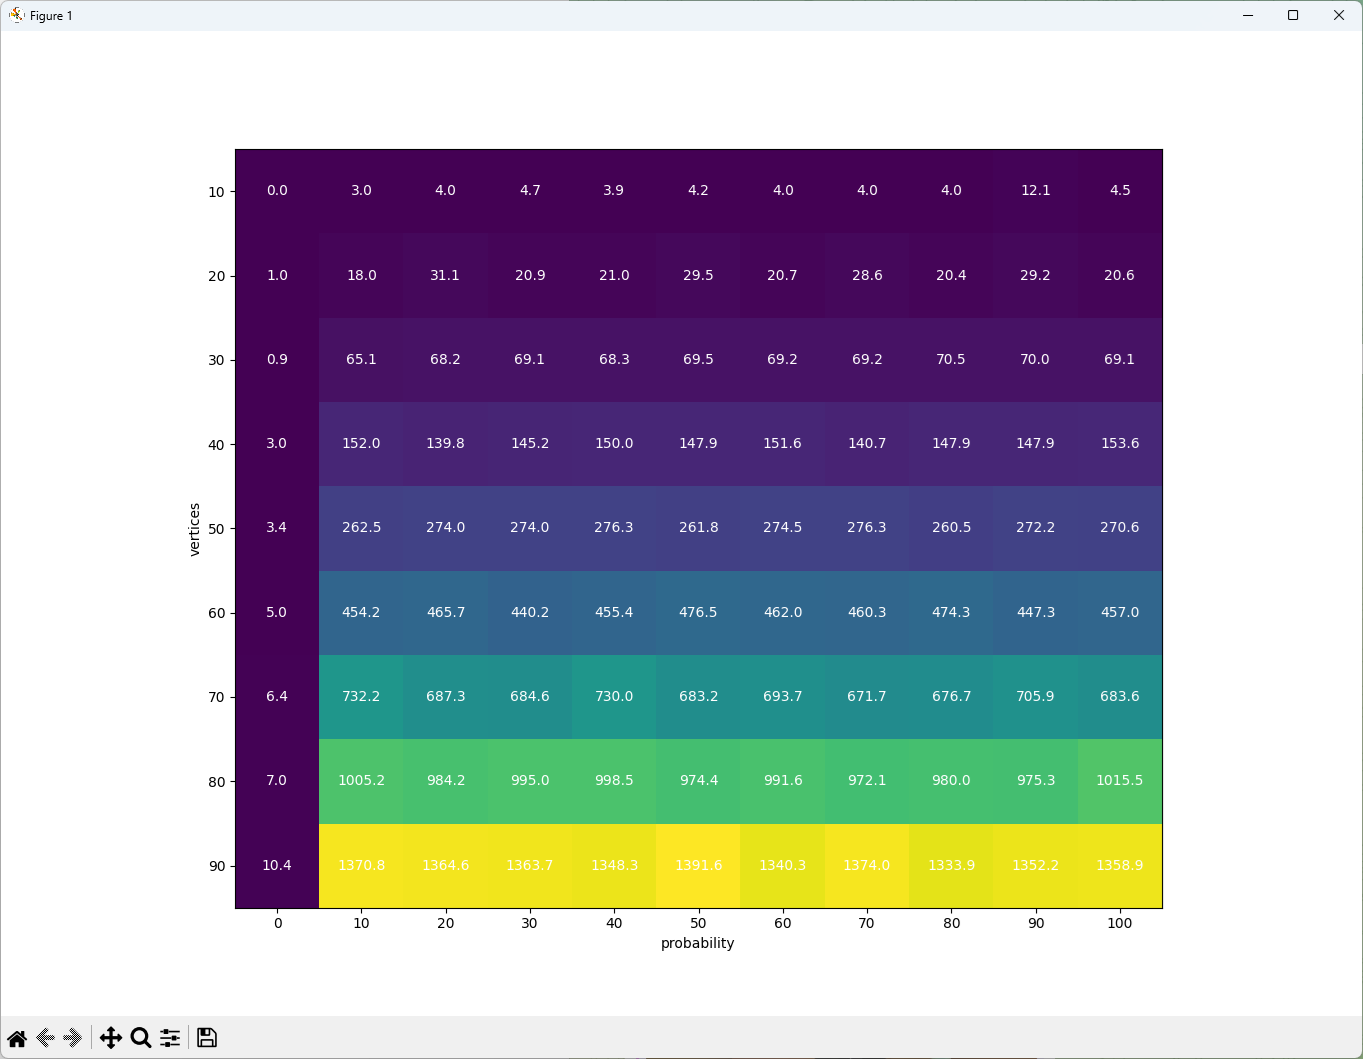
\includegraphics[width=125mm]{toll}
\end{center}\indent

Явно видно, що за відсутності ребер складність O(n). Час роботи залежить від кількості вершин значно більше ніж від кількості наявних ребер: можна знехтувати кількістю ребер та сказати що складність роботи залежить виключно від кількості вершин. Складність перетворення матричної форми. Отримана складність -- O($n^2$), очікувана складність залежить виключно від кількості ребер. При використанні об'єктів list, замість списків, для списків суміжності можна було б покращити час роботи.
\newpage

Результати тестування \textit{from\_ll}:
\begin{center}
    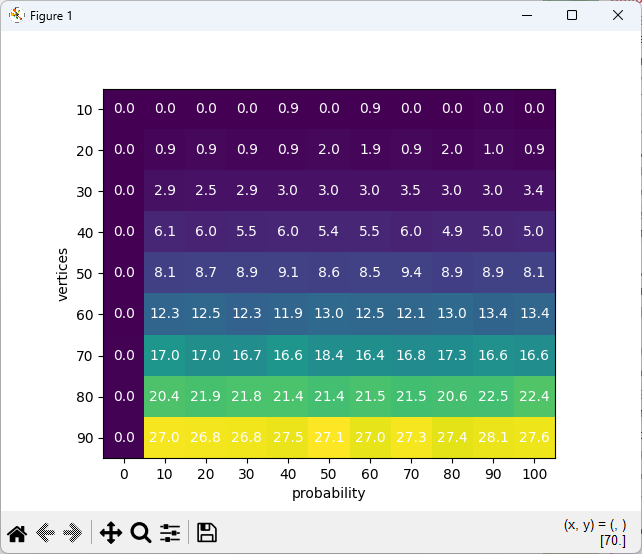
\includegraphics[width=125mm]{fromll}
\end{center}\indent

Явно видно, що за відсутності ребер складність O(1). При наявності ребер складність O($n^2$). Очікувана складність залежить від кількості ребер.\\\indent

Додаткові тестування перетворень з ймовірністю ребер від 0 до 10 показують, що час роботи не залежить від ймовірності якщо вона більше 5\% і час роботи наближається до нуля якщо ймовірність наближається до 0\%. Додаткові тестування з більшою кількістю вершин показують, що час роботи не залежить від ймовірності, якщо ймовірність більше або рівна 1\%, на графах з більш ніж 400 вершинами. Можна зробити висновок, що складність роботи перетворень матриць суміжностей на списки, та навпаки, має середню складність O($n^2$) та не залежить від кількості ребер. \\\indent
 Viva Python та його "швидкодія" яка перетворює адекватні алгоритми на алгоритми з експоненційною складністю.\\\\\indent
Посилання на репозиторій практикуму:\\ \href{$https://github.com/MINIAProgramStudio/applied_algorythms/tree/main/task_2$}{$https://github.com/MINIAProgramStudio/applied\_algorythms/tree/main/task\_2$}\sloppy

\end{document}